\chapter{Analyse}
In diesem Kapitel werden die in Kapitel \ref{ch:konzeption} vorgestellten Systeme analysiert.

\section{128MB Konfigurationen}
Zunächst werden alle Tests für die 128MB Konfigurationen ausgeführt. In der folgenden Sektionen wird dann die Speicher- und Prozessorgröße erhöht. 

\subsection{Pipe-Clean Tests}
Zunächst wird die Performance der \acp{SUT} in der bestmöglichen Situation mit einem einzigen Nutzer ermittelt. Ziel dessen ist es, eine Vergleichsgrundlage für die darauf folgenden Tests zu schaffen. Die Tests wurden mit einer Dauer von zehn Minuten und einem aktiven Benutzer für jeden Use-Case durchgeführt.

\begin{figure}[H]
    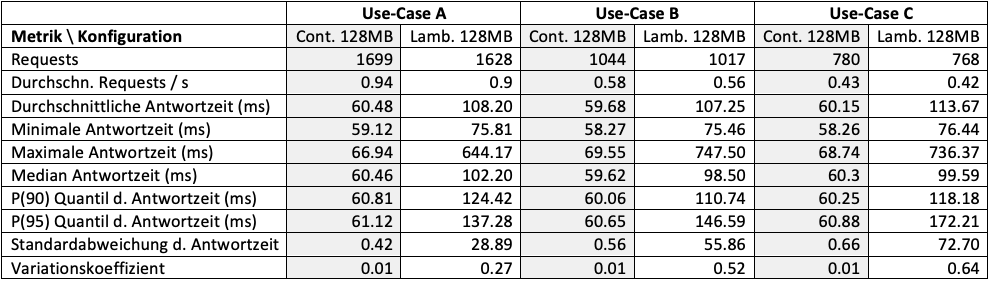
\includegraphics[width=\textwidth]{img/pipe128-comparison.png}
    \caption[Vergleich der Pipe-Clean Tests für 128MB]{Vergleich der Pipe-Clean Tests für 128MB}
    \label{fig:pipe128-comparison}
\end{figure}

Abbildung \ref{fig:pipe128-comparison} zeigt die Ergebnisse des Tests für die Funktionen mit 128MB CPU bzw. RAM. Die Zahlen sind in der Tabelle aufgrund des Testing-Tools in der Notation mit Punkt anstatt eines Kommas angegeben. Es ist zu erkennen, dass die Container-Anwendung in allen Fällen eine deutlich geringere Antwortzeit als die Lambda-Anwendung aufweist. Im Median ist der Container bei Use-Case A etwa 41,74ms schneller als die Lambda-Funktion. Die Lambda-Anwendung weist eine überaus große Varianz in ihren Antwortzeiten auf, was in ihrer Standardabweichung und einem Variationskoeffizient von bis zu 0,64 deutlich wird, während dieser bei der Container-Anwendung in allen drei Use-Cases bei nur 0,01 liegt. Die Antwortzeit der Lambda-Anwendung im Median liegt jedoch in allen drei Use-Cases bei ähnlichen Werten um ca. 100ms. Andererseits nimmt die Abweichung vom Mittelwert und das P(95) Quantil der Antwortzeit bei Use-Case B im Vergleich zu Use-Case A deutlich zu. Auch bei Use-Case C ist ein deutlicher Anstieg der Werte zu beobachten. Vermutlich ist dies auf die größere Anzahl an angefragten Endpunkten zurückzuführen, da dadurch mehr Coldstarts durchgeführt werden mussten. 
Auch bei der Container-Anwendung ist keine Veränderung der Median-Antwortzeit zwischen den einzelnen Use-Cases festzustellen, da sie sich in allen Tests um einen Wert von ca. 60ms bewegt. Die Standardabweichung der Antwortzeit veränderte sich mit eine Erhöhung von 0,42 auf 0,66 zwischen Use-Case A und C nur leicht. Der Variationskoeffizient blieb aber in allen drei Use-Cases bei 0,01.

Anhand der Vergleichstabelle lassen sich auch Erkenntnisse über die einzelnen Use-Cases ableiten. Use-Case A setzt sowohl bei der Container- als auch bei der Lambda-Anwendung deutlich mehr Requests in der Sekunde ab als es bei den Use-Cases B und C der Fall ist. Dies ist auf die größeren Think-Times von drei Sekunden zurückzuführen, wie sie bei den Use-Cases mit Benutzer-Eingaben zum Einsatz kommt.

\subsection{Stress-Tests}
Um \hyperref[tab:research-questions]{RQ1} beantworten zu können, muss zunächst die maximale Auslastung eines einzelnen Containers ermittelt werden. Dazu werden mehrere Stress-Tests durchgeführt. Ein Stress-Test dient dazu, die Grenzen des \ac{SUT} herauszufinden. Da Lambda ein von Natur aus automatisch horizontal skalierendes System ist, werden die Test zunächst für die Container-Anwendung durchgeführt und im Anschluss die Lambda-Anwendung mit dem gleichen Test-Ablauf getestet. Die Anzahl der \acp{VU} wird bei den Stress-Tests, wie von Molyneaux\cite{molyneaux_art_2014} empfohlen, immer stufenweise erhöht. Das bedeutet, dass nach jedem linearer Anstieg, auch Ramp-Up genannt, eine gleichlange Periode mit einer konstanten Anzahl an Benutzern folgt. Abbildung \ref{fig:stress-vus-example} verdeutlicht dies anhand eines Stress-Tests, bei dem bis zu 600 gleichzeitige Virtuelle Benutzer erstellt werden. In 60 Sekunden Zeitabschnitten werden nach und nach immer 60 Benutzer hinzugefügt. Daraufhin folgt eine weitere 60 Sekunden lange Periode, in der die Anzahl der \acp{VU} nicht weiter erhöht wird. Der gesamte Test hat demnach eine Dauer von 40 Minuten. Eine Cooldown-Phase, bei der die Anzahl der Benutzer nach Erreichen des Limits langsam zurückgefahren wird, wird hier nicht eingelegt, da das Verhalten der Systeme beim Herunterskalieren nicht untersucht werden soll.

\begin{figure}[H]
    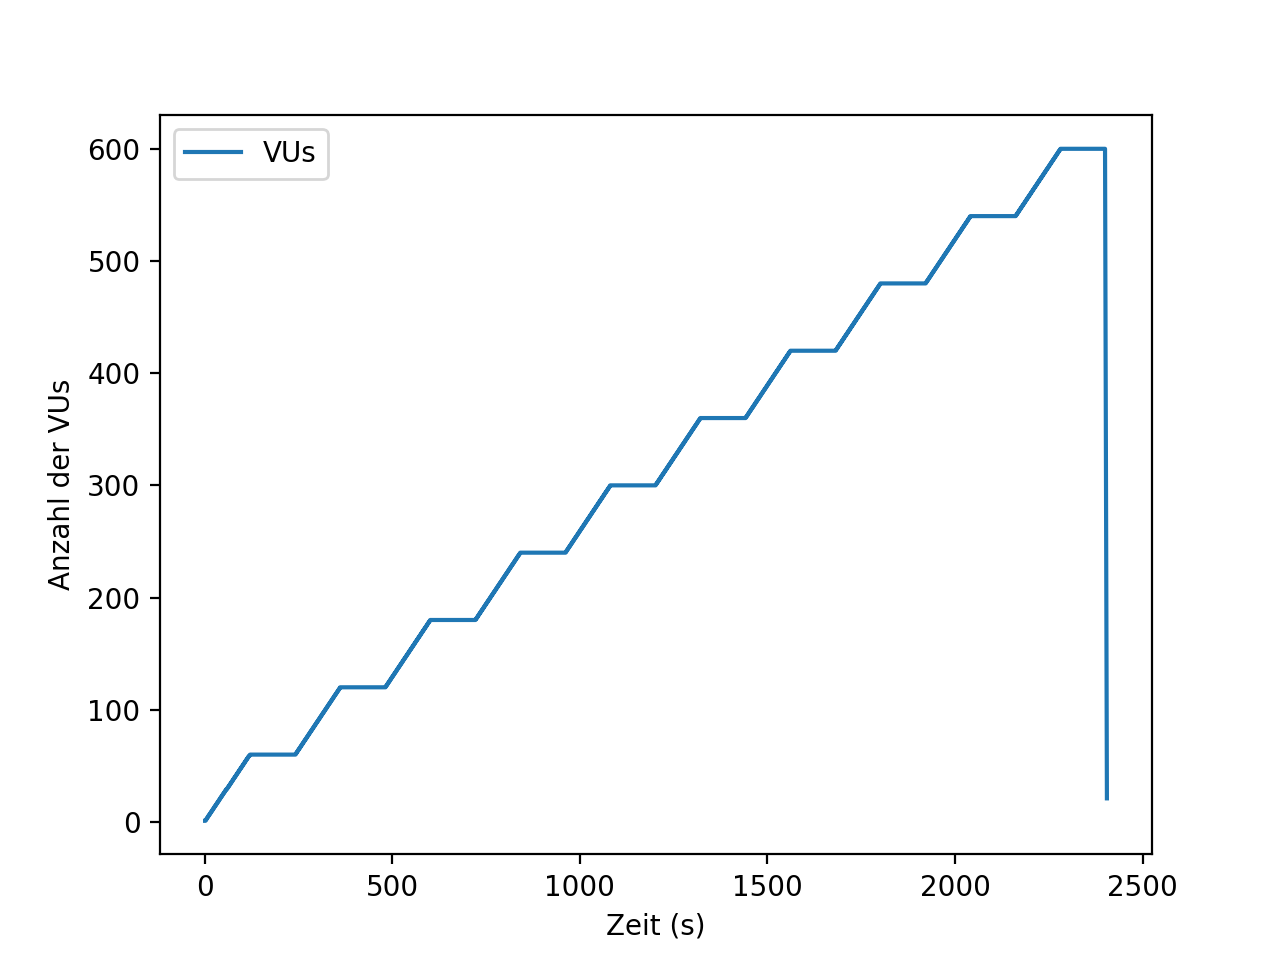
\includegraphics[width=\textwidth]{img/stress-vus-example.png}
    \caption[Beispiel-Anstieg der gleichzeitigen VUs für einen Stress-Test]{Beispiel-Anstieg der gleichzeitigen VUs für einen Stress-Test}
    \label{fig:stress-vus-example}
\end{figure}

\subsubsection{Container}
Für die containerisierte Anwendung in der 128MB Konfiguration wurden mehrere Stress-Tests durchgeführt, bis das Limit der gleichzeitigen Benutzer identifiziert werden konnte. Abbildung \ref{fig:fargate128-stress-comparison} zeigt die gemessenen Metriken für die einzelnen Use-Cases und Stress-Test Konfigurationen. 

\begin{figure}[H]
    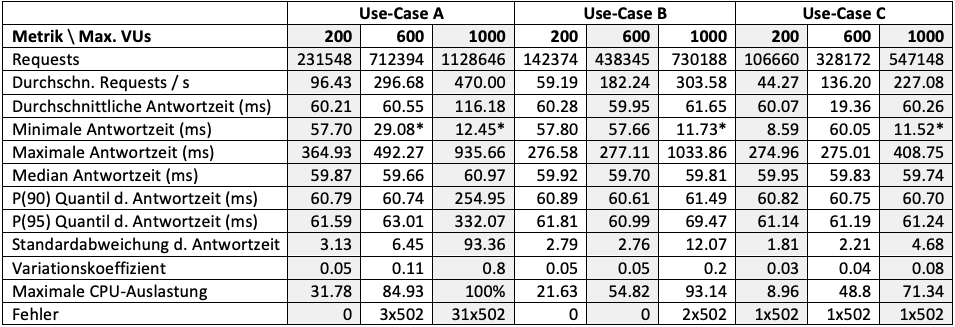
\includegraphics[width=\textwidth]{img/fargate128-stress-comparison.png}
    \caption[Container 128MB Stress-Test Vergleich]{Container 128MB Stress-Test Vergleich}
    \label{fig:fargate128-stress-comparison}
\end{figure}

Der erste Test wurde mit bis zu 200 Benutzern durchgeführt. Dabei konnte bei Use-Case A nicht einmal 32\% CPU-Auslastung des Container-Clusters erreicht werden; Bei Use-Case B waren es sogar unter 22\%. Der geringen Auslastung entsprechend, war kaum eine Veränderung der Antwortzeiten gegenüber den Pipe-Clean Tests festzustellen (vgl. mit Abbildung \ref{fig:pipe128-comparison}). Einige Metriken lagen sogar unter den Grundwerten. Lediglich die maximale Antwortzeit hat sich bei allen Use-Cases deutlich erhöht, bspw. bei Use-Case A von 60,46ms auf 558,12ms. Diese Erhöhungen sind allerdings nur vereinzelt der Fall, da immer noch 95\% aller Anfragen innerhalb 62ms beantwortet wurden. Der Variationskoeffizient stieg bei allen Use-Cases leicht an. 

Bei dem zweiten Stress-Test mit bis zu 600 \acp{VU}, änderte sich nicht viel im Vergleich zu dem Test mit 200 Benutzern. Es konnten für Use-Case A zwar bis zu 84,93 Prozent CPU-Auslastung erreicht werden und die maximale Antwortzeit stieg erneut an auf 638,19ms. Trotz dessen, konnten von dem einzelnen Container erneut 95\% der Anfragen innerhalb von 62ms beantwortet werden. Bei Use-Case A fallen fünf Requests auf, die vom Server nicht beantwortet werden konnten und den HTTP 502 Fehlercode zurücksendeten. Dies entspricht jedoch nur einem äußerst geringen Anteil aller in diesem Stress-Test durchgeführten Anfragen. Bei Use-Case B trat nur ein Fehler auf, bei Use-Case C waren es vier.

\begin{figure}[H]
    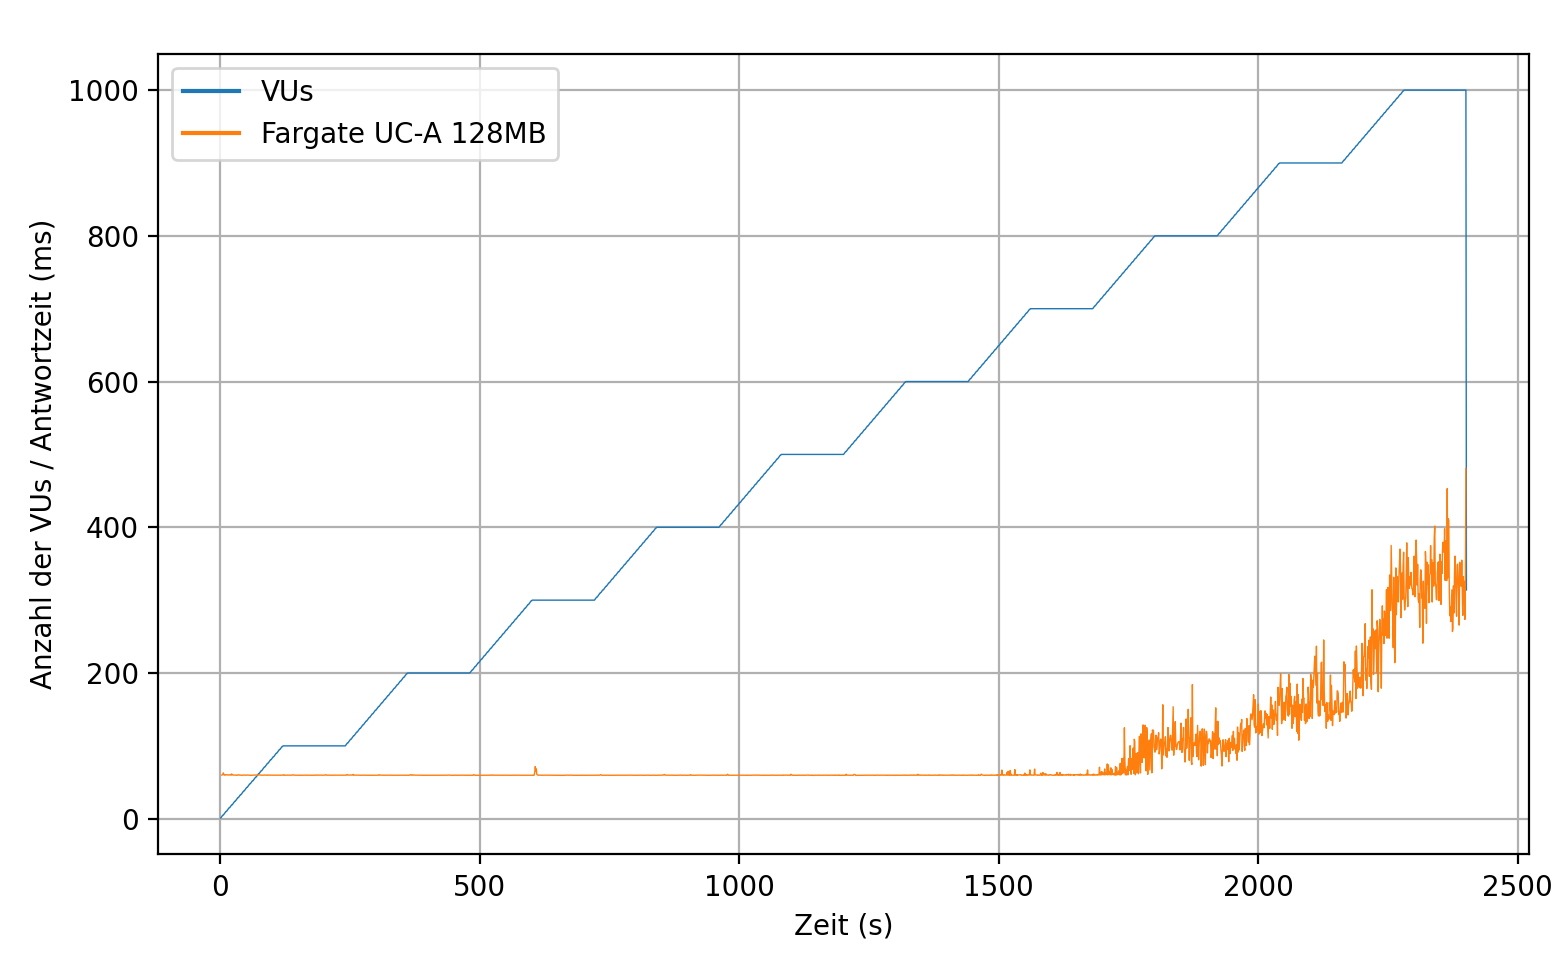
\includegraphics[width=\textwidth]{img/fargate128-stress1000-uca-example-graph.png}
    \caption[Container Use-Case A 128MB Stress-Test mit 1000 VUs Verlauf Vergleich]{Container Use-Case A 128MB Stress-Test mit 1000 VUs Verlauf Vergleich}
    \label{fig:fargate128-stress1000-uca-example-graph}
\end{figure}

Der dritte Stress-Test für den 128MB Container wurde mit bis zu 1.000 \acp{VU} durchgeführt. Abbildung \ref{fig:fargate128-stress1000-uca-example-graph} zeigt den zeitlichen Verlauf eines der beiden Tests für Use-Case A. Es wird dabei die Anzahl der virtuellen Benutzer und die Antwortzeit im Median pro Sekunde dargestellt. Es wird deutlich, dass die Antwortzeit ab ca. 700 \acp{VU} deutlich ansteigt. Dies deckt sich der von \ac{AWS} Cloudwatch gemessenen CPU-Auslastung von 100\% die bei dieser Nutzerzahl gemessen wurde. In den darauf folgenden Perioden mit Anstieg der \acp{VU} steigt auch die Antwortzeit. In jeder Periode mit konstanten Nutzerzahlen können die Requests besser verarbeitet werden und die Kurve geht wieder leicht herunter. Während des Tests wurden trotz einer vollen CPU-Auslastung nur 77 HTTP 502 Fehlercodes vom Server ausgelöst, was einer Quote von 0,003\% entspricht. Die durch Fehler hervorgerufenen Werte sind in allen Tabellen-Abbildungen mit einem Asterisk (*) gekennzeichnet. Die Antwortzeit konnte im Median weiterhin bei etwa 60ms gehalten werden; die durchschnittliche Antwortzeit stieg mit 108,65ms auf fast das doppelte des Grundwertes an.
Bei Use-Case B lag die erreichte Prozessor-Auslastung bei 94,99\%. Es wurden bis auf acht HTTP 502 Fehlercodes keine deutlichen Abweichungen von den Pipe-Clean Tests ausgelöst. Der Variationskoeffizient stieg mit 0,16 leicht an, liegt aber immer noch deutlich unter dem Wert des Pipe-Clean Tests der 128MB Lambda-Funktion. Der Wertanstieg könnte durch die von den aufgetretenen Fehler verursachten geringen Antwortzeiten von bis zu 11,73ms ausgelöst worden sein sein. 
Um die maximale Auslastung des Containers für die anderen beiden Use-Cases zu erreichen, wurden noch weitere Stress-Tests mit bis zu 1.500 \acp{VU} durchgeführt. Bei Use-Case B konnte das Limit zwischen 1.000 und 1.100 Benutzern erreicht werden. Für Use-Case C liegt es bei ca. 1.200-1.300 Benutzern. Dadurch dass sich das Limit zwischen den beiden Ausführungen des gleichen Tests leicht unterscheiden kann, müssen hier Wertebereiche angegeben werden.

\subsubsection{Lambda}
Nachdem die maximale Performance des 128MB Containers ermittelt wurde, werden im Anschluss die gleichen Stress-Tests für die Lambda-Anwendung mit 128MB durchgeführt. Abbildung \ref{fig:lambda128-stress-comparison} zeigt die Ergebnisse der Tests. 
Allgemein liegt die Antwortzeit im Median immer noch deutlich über der des 128MB Containers; die Differenz ist allerdings im Vergleich zu den Pipe-Clean Tests gesunken, bspw. von 41,74ms auf 17,72ms bei den Tests mit bis zu 1.000 \acp{VU} für den ersten Use-Case.
Für Use-Case A lässt sich ebenfalls erkennen, dass die Standardabweichung bei 200 und 600 \acp{VU} noch um die 18 beträgt, während sie bei 1.000 Usern auf ca. 41 ansteigt. Auch der Variationskoeffizient stieg von ca. 0.2 auf 0.47 an. Dies könnte allerdings an den extrem langen maximalen Antwortzeiten von bis zu 29.037ms liegen, die durch die aufgetretenen Fehler verursacht wurden. Die großen Fehler-Latenzen stehen im Gegensatz zu der Container Anwendung, bei der die maximale Antwortzeit nur knapp über einer Sekunde lag. Auffallend ist, dass Fehler mit HTTP Statuscode 500 etwa 10 Sekunden Antwortzeiten aufweisen, während Fehler mit HTTP Statuscode 504 die fast 30 Sekunden lange Latenz erzeugen. Die bei der Container-Anwendung erzeugten HTTP 502 Fehlercodes, führten zu kleineren Antwortzeiten von 12ms bis zu 260ms. 

\begin{figure}[H]
    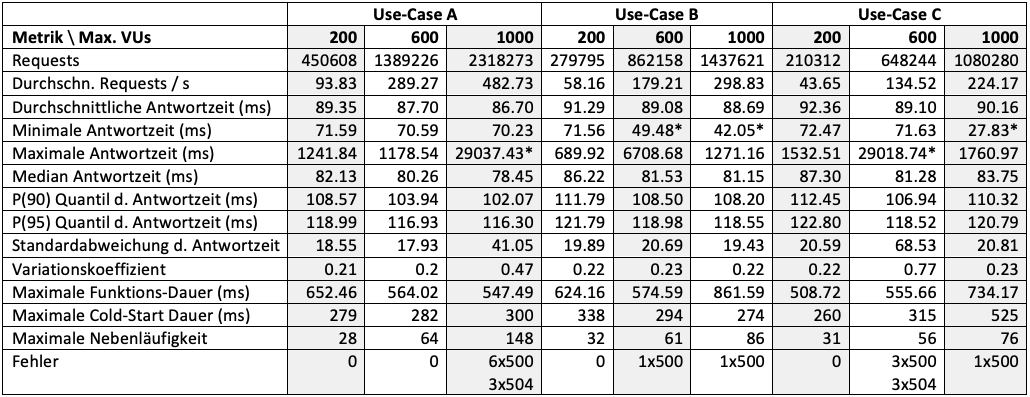
\includegraphics[width=\textwidth]{img/lambda128-stress-comparison.png}
    \caption[Lambda 128MB Stress-Test Vergleich]{Lambda 128MB Stress-Test Vergleich}
    \label{fig:lambda128-stress-comparison}
\end{figure}

Bei der Durchführung der Stress-Tests für die 128MB Lambda-Anwendung fällt außerdem auf, dass die Antwortzeit im Median bei steigenden Nutzerzahlen zu sinken scheint. Bei bis zu 200 \acp{VU} lag sie für Use-Case A noch bei 83.13ms, während sie bei bis zu 1.000 \acp{VU} auf 78.45ms sank. Die Werte für Use-Case B und C scheinen auch zwischen dem ersten und zweiten Stress-Tests zu sinken, zwischen 600 und 1.000 \acp{VU} gab es aber keinen Unterschied mehr in den Antwortzeiten. Die deutlich höhere Request-Rate von Use-Case A lässt darauf schließen, dass \ac{AWS} die Funktionen schneller provisioniert, je mehr Anfragen sie erhalten.
Dies würde auch den Verlauf aus Abbildung \ref{fig:lambda128-stress1000-comparison-graph} erklären, bei dem jeweils eine Test-Ausführung der drei Use-Cases für den Stress-Test mit bis zu 1.000 Benutzern abgebildet ist.

\begin{figure}[H]
    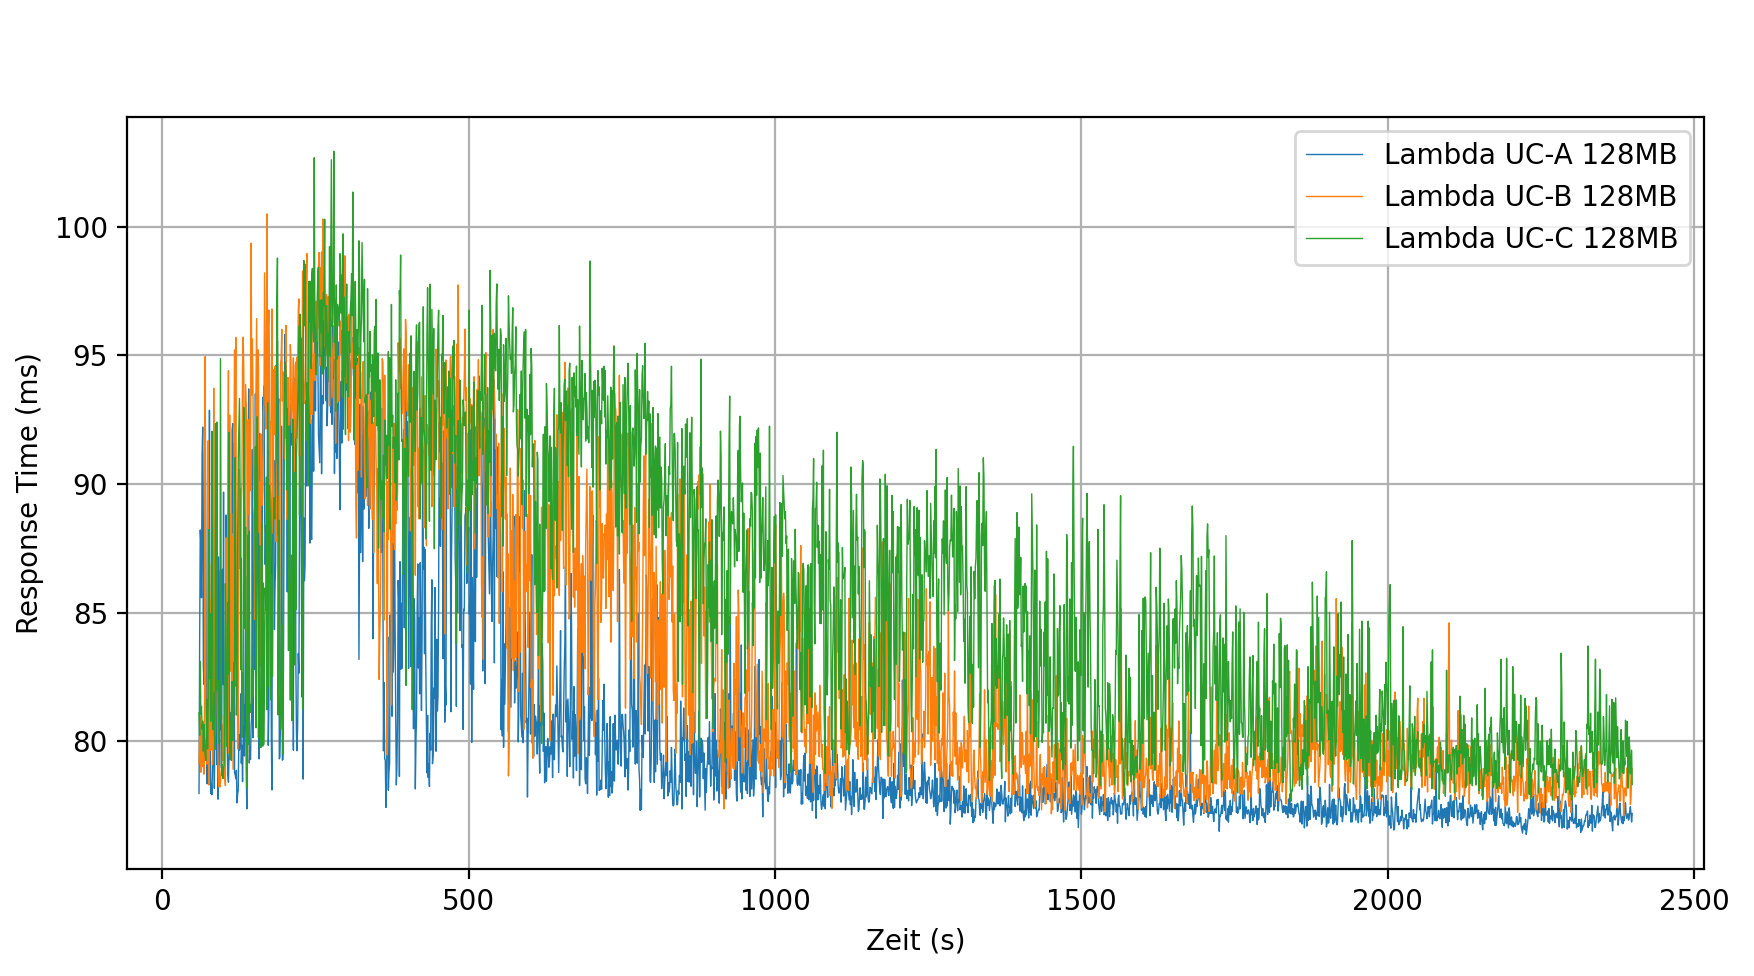
\includegraphics[width=\textwidth]{img/lambda128-stress1000-comparison-graph.png}
    \caption[Lambda 128MB Stress-Test mit 1.000 VUs Verlauf Vergleich]{Lambda 128MB Stress-Test mit 1.000 VUs Verlauf Vergleich}
    \label{fig:lambda128-stress1000-comparison-graph}
\end{figure}

Aus Gründen der Übersichtlichkeit wurde der Graph erst ab einer Minute dargestellt, da bei den Lambda-Funktionen vor allem in den ersten Sekunden der Tests verhältnismäßig hohe Response-Times auftreten. Es ist zu erkennen, dass die Antwortzeiten bei allen Use-Cases am Anfang ansteigen und nach ca. 300 Sekunden ihren Höhepunkt bei in etwa 95 bis 100ms erreichen. Danach flachen alle Kurven langsam ab, bis sie sich einem Wert von etwas unter 80ms annähern. Dabei scheint die Kurve von Use-Case A jedoch steiler als die von Use-Case B abzuflachen. Und auch dieser befindet sich schneller auf einem niedrigeren Niveau als der dritte Anwendungsfall.

Die höhere Request-Rate von Use-Case A macht sich ebenfalls in der Anzahl der nebenläufigen (concurrent) Lambda-Funktionen bemerkbar. Während bei 200 \acp{VU} für Use-Case B und C noch mehr Funktionen bereitgestellt wurden als für Use-Case A, zeigt sich für 600 und 1.000 \acp{VU} ein umgekehrtes Bild. Dort übertrifft der erste Use-Case den die anderen beiden deutlich in der Anzahl der nebenläufigen Funktionen. 

\subsection{Load-Tests}
Für \hyperref[tab:research-questions]{RQ2} soll die Performance unter normalen Nutzerzahlen mit der von schnell ansteigenden Nutzerzahlen verglichen werde. Dazu wird zunächst ein Load-Test für die in den vorangegangenen Stress-Tests ermittelten Nutzer-Grenzen der Container-Anwendung durchgeführt. Im Anschluss wird ein Spike-Test mit der gleichen Benutzerzahl durchgeführt. Ziel dessen ist es, die Performance der Anwendungen unter rasch ansteigender Last zu ermitteln. 

In den bisherigen Stress-Tests wurden nur langsame Anstiege (Ramp-Ups) durchgeführt. Für den Container wurde eine maximale Belastbarkeit von ca. 700 Benutzern ermittelt. Deshalb wird nun für den Load-Test von einem normalem Load von 600 Benutzern ausgegangen, um den Container nicht zu stark zu belasten.

\begin{figure}[H]
    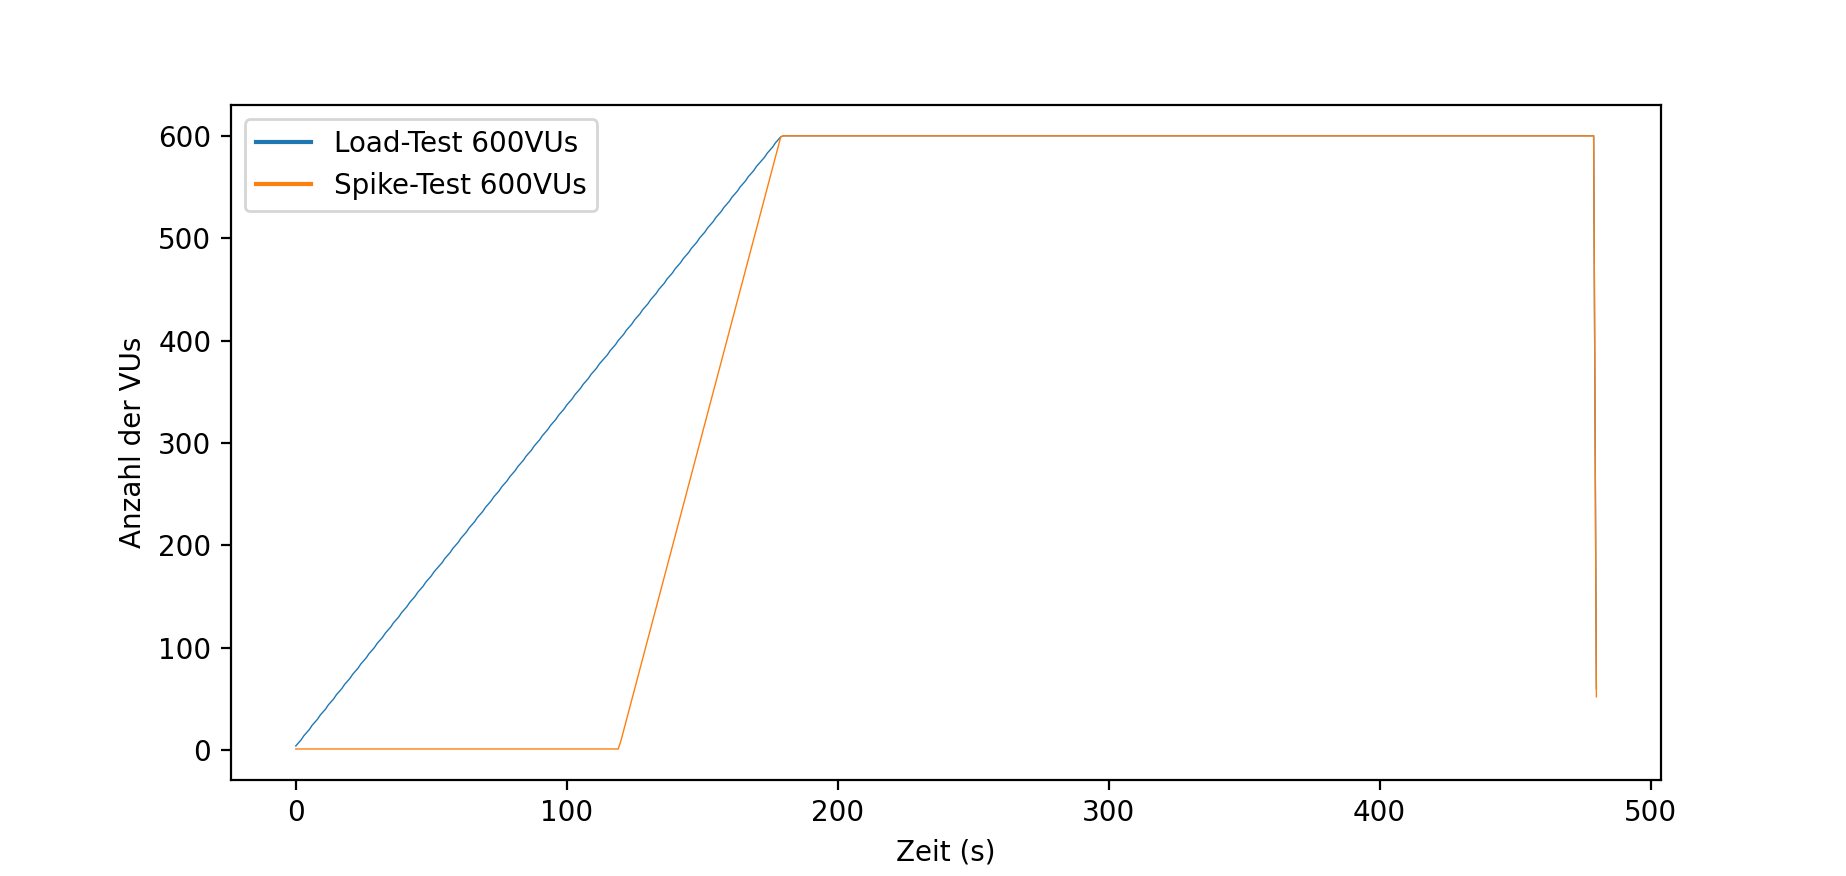
\includegraphics[width=\textwidth]{img/load600-vs-spike600.png}
    \caption[Load- und Spike-Test mit 600 VUs Vergleich]{Load- und Spike-Test mit 600 VUs Vergleich}
    \label{fig:load600-vs-spike600}
\end{figure}

Abbildung \ref{fig:load600-vs-spike600} zeigt die unterschiedlichen Test-Verläufe der beiden Tests. Die Anzahl der Benutzer steigt bei dem Load-Test von Anfang an kontinuierlich an und erreicht innerhalb von drei Minuten die maximale Grenze. Für den Spike-Test erfolgt nach einer zwei-minütigen Warte-Phase, in der keine Benutzer auftreten, ein schneller Anstieg innerhalb von einer Minute auf die 600 \acp{VU}. Der Anstieg des Spike-Tests ist also drei mal steiler als der des Load-Tests. 
Nach Erreichen der Obergrenze wird bei beiden Tests die Anzahl der Benutzer für fünf Minuten konstant gehalten. Dies lässt eventuelle Nachwirkungen des Anfrage-Ansturms erkennen.


\subsubsection{Container}
Bei der Durchführung der Tests für den 128MB Container konnten keine Veränderungen der Performance für einen schnellen Anstieg der Benutzer gegenüber dem langsamen Anstieg festgestellt werden. Für alle Use-Cases lag der Median der Antwortzeit knapp unter 60ms. Neunzig Prozent aller Requests wurden unter 62ms verarbeitet, das P(95) Quantil lag auch meist bei diesem Wert. Allein bei Use-Case A kam es zu erhöhten Werten von 65 bzw. 67ms bei den Load-Tests und fast 70ms bei den Spike-Tests. Dies ist vermutlich erneut auf die höhere Request-Rate des ersten Use-Case zurückzuführen.

Die Varianz veränderte sich stark zwischen den unterschiedlichen Test-Läufen. Der Wert von 0,01 aus den Pipe-Clean Tests wurde deutlich übertroffen. Use-Case C wies mit 0,05 und 7,39 den sowohl kleinsten als auch größten Wert der Load-Tests auf. Der letztere wurde durch einen starken Ausreißer verursacht, bei dem eine Zeit von fast 28 Sekunden verging, bevor die Antwort des Services registriert wurde. Bei den Spike-Tests lagen alle Werte der Use-Cases mit mehreren Endpunkten zwischen 0,04 und 0,08. Use-Case A wies Werte von 0,13 und 0,14 auf und lag damit deutlich vor den anderen getesteten Anwendungsfällen. Verursacht wurde dies vermutlich durch jeweils einen HTTP 502 Fehler, der die minimale Antwortzeit auf 16,28 bzw. 13,46ms schrumpfen ließ. Bei den anderen Use-Cases traten in den Spike-Tests keine Fehler auf.

\subsubsection{Lambda}
Bei den Lambda-Funktionen lassen sich für Use-Case A keine eindeutigen Unterschiede in der Antwortzeit für die beiden verschiedenen Anstiegs-\linebreak Intervalle feststellen. In den beiden Load-Tests wurden 50 Prozent aller Requests in 80,24ms bzw. 84,49ms erledigt. Bei den Spike-Tests waren es 79,97ms bzw. 85ms. Im ersten Lauf der Load-Tests wurde eine maximale Nebenläufigkeit von 72 Funktionen festgestellt, im zweiten waren es 67. Bei den Spike-Tests waren es 67 und 68.

Abbildung \ref{fig:lambda-uca-load600-vs-spike600-example} zeigt ein Vergleich jeweils eines Load- und Spike-Tests für Use-Case A. Für den Load-Tests (blaue Linie) ist zu erkennen, dass sich nach anfänglich hohen Antwortzeiten von ca. 95ms das Niveau bei 75 bis 80ms einpendelt. Ab 180 Sekunden (3 Minuten) ist bei beiden Tests die maximale User-Anzahl erreicht. Nach ca. 200 Sekunden überschreitet die Median-Antwortzeit für den Load-Test die 80ms Marke und erreicht ihren Höchststand nach ca. 350 Sekunden mit ca. 90ms. Danach sinkt die Median-Antwortzeit wieder trotz konstanter Nutzerzahlen.
Für den Spike-Test scheint es sich ähnlich zu verhalten. Auch wenn nach 180 Sekunden die 600 \acp{VU} erreicht wurden, klettert die Antwortzeit erst mehr als eine Minute später über die 80ms Marke. Der Spike-Test erreicht ebenso wie der Load-Test nach ca. 350 Sekunden sein Maximum; dessen Antwortzeit liegt mit ca. 93ms nur leicht über der des Load-Tests.

\begin{figure}[H]
    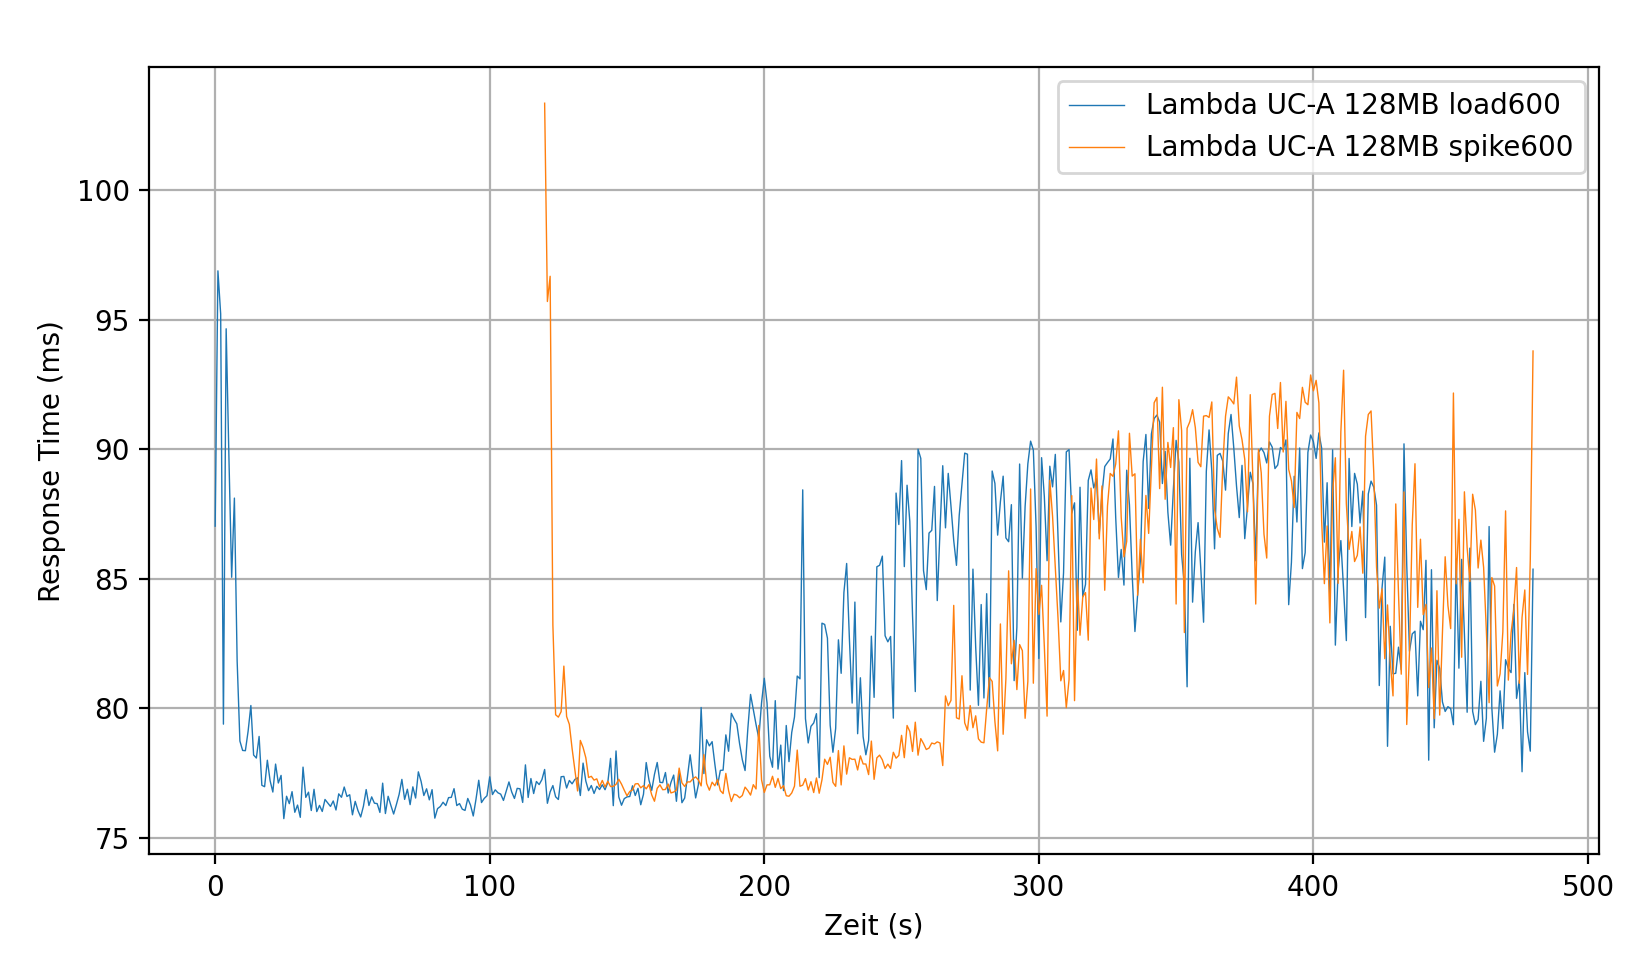
\includegraphics[width=\textwidth]{img/lambda-uca-load600-vs-spike600-example-new.png}
    \caption[Lambda Use-Case A Load- und Spike-Test mit 600 VUs Verlauf Vergleich]{Lambda Use-Case A Load- und Spike-Test mit 600 VUs Verlauf Vergleich}
    \label{fig:lambda-uca-load600-vs-spike600-example}
\end{figure}

Für Use-Case B (Abbildung \ref{fig:lambda-ucb-load600-vs-spike600-example}) wurden zwei stark unterschiedliche Verläufe der Load-Tests festgestellt. Der erste Load-Test (blaue Linie) zeigt einen flacheren Verlauf als der zweite (orange Linie). Seine Kurve fällt nach Erreichen der höchsten Antwortzeit bei ca. 90ms schneller ab. Zudem liegt die maximale Antwortzeit des zweiten Load-Tests mit ca. 95ms in etwa 5ms über der des ersten. Auch der Spike-Test (grüne Linie) erreicht eine maximale (Median-)Antwortzeit von ca. 95ms, womit dessen Verlauf stärker dem zweiten Load Test ähnelt. 

\begin{figure}[H]
    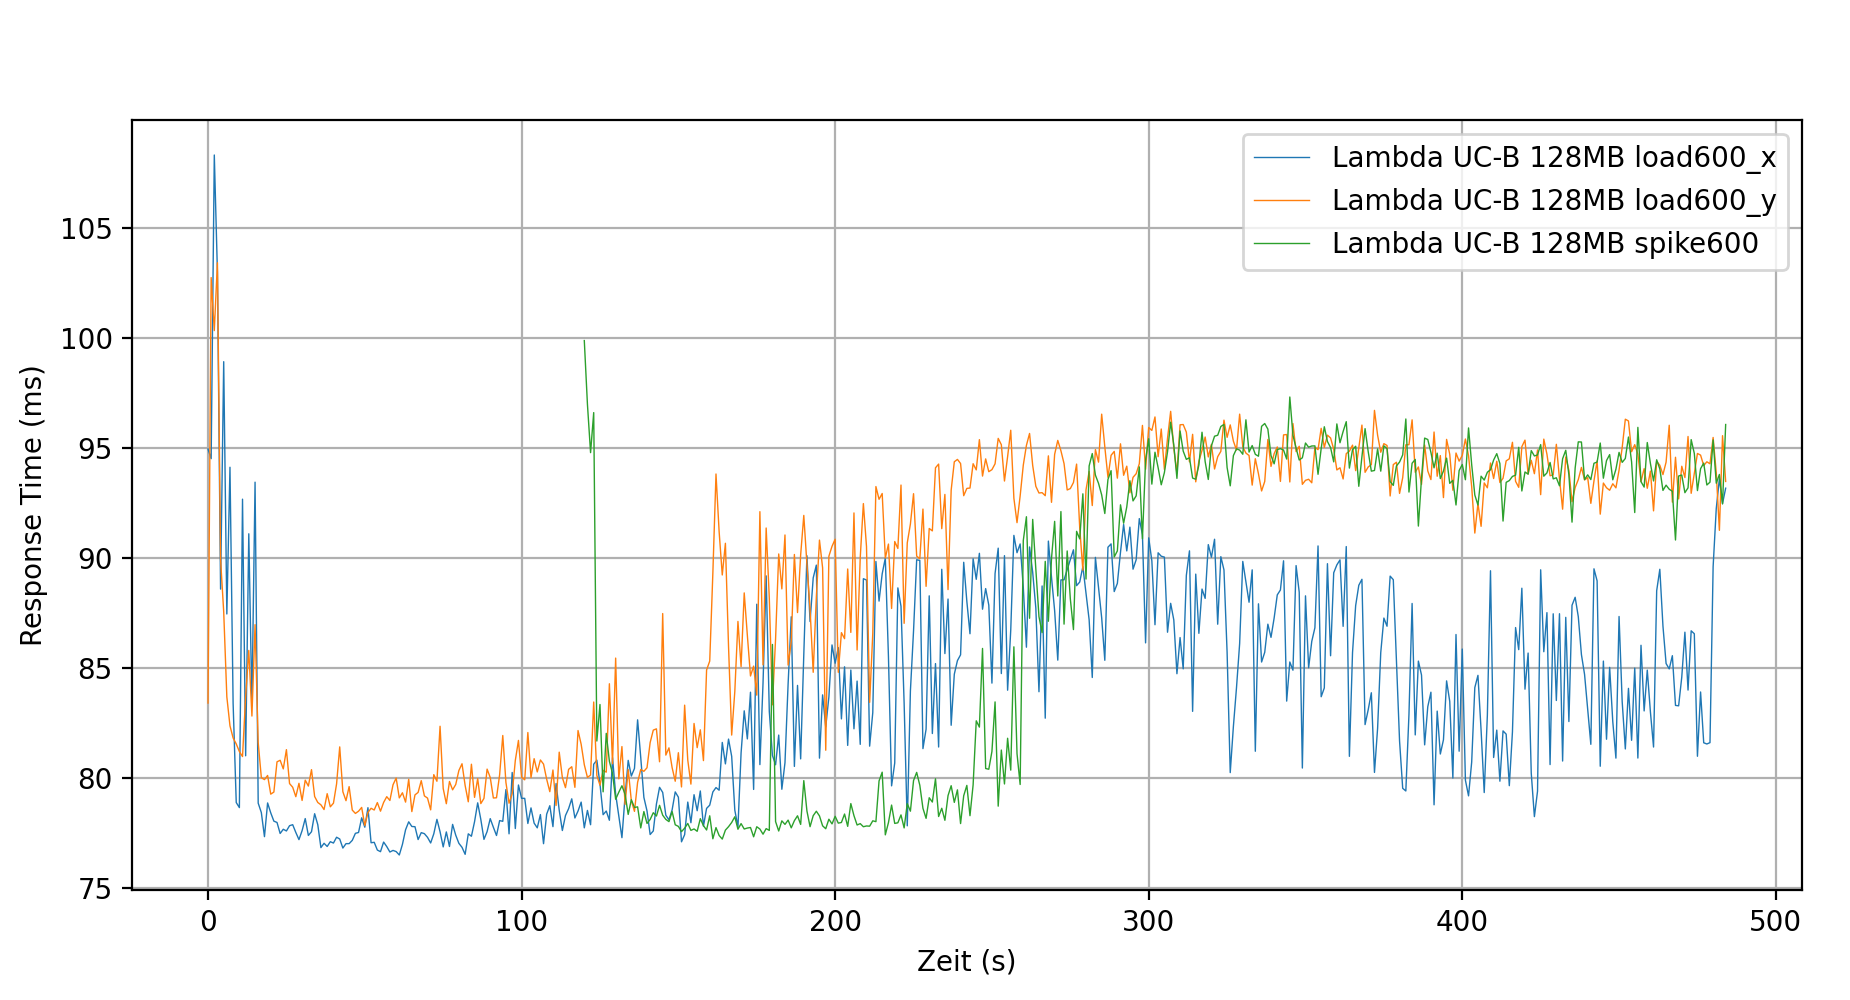
\includegraphics[width=\textwidth]{img/lambda-ucb-load600-vs-spike600-example2.png}
    \caption[Lambda Use-Case B Load- und Spike-Test mit 600 VUs Verlauf Vergleich]{Lambda Use-Case B Load- und Spike-Test mit 600 VUs Verlauf Vergleich}
    \label{fig:lambda-ucb-load600-vs-spike600-example}
\end{figure}

Es wird deutlich, wie unterschiedlich die Verläufe eines identischen Tests bei der Lambda-Anwendung ausgeprägt sein können. Interessant ist außerdem, dass die Antwortzeit des ersten Load-Test eine größere Schwankung aufweist, als die des zweiten und des Spike-Tests, bei denen aufeinander folgende Werte stets relativ nah beieinander liegen. Aufgerufen wurden bei den Load-Tests jeweils 60 Funktionen, bei den Spike-Tests waren es 66 bzw. 62 Instanzen.

Auch bei Use-Case C konnte keinen großen Unterschiede zwischen den Load- und Spike-Tests mit 600 \acp{VU} festgestellt werden. In allen Tests wurden Median-Antwortzeiten von 86 bis 90ms gemessen. Hier wurden bei den Load-Tests 58 bzw. 56 und bei den Spike-Tests 58 bzw. 57 Funktionen parallel aufgerufen.
Da die Antwortzeiten der Spike-Tests in allen Fällen trotz des dreimal steileren Anstiegs äußerst nah bei denen der Load-Tests liegen, ist daraus zu schließen, dass ein schneller Spike-Load nur eine geringfügige Veränderung der Antwortzeit mit sich bringt. 

Es zeichnet sich wie auch schon bei den Stress-Tests ein Unterschied der Antwortzeiten zwischen den einzelnen Use-Cases ab. Exemplarisch zeigt Abbildung \ref{fig:lambda128-load600-uc-comparison} den Verlauf der Antwortzeiten im Median für den Load-Test mit bis zu 600 \acp{VU}.

\begin{figure}[H]
    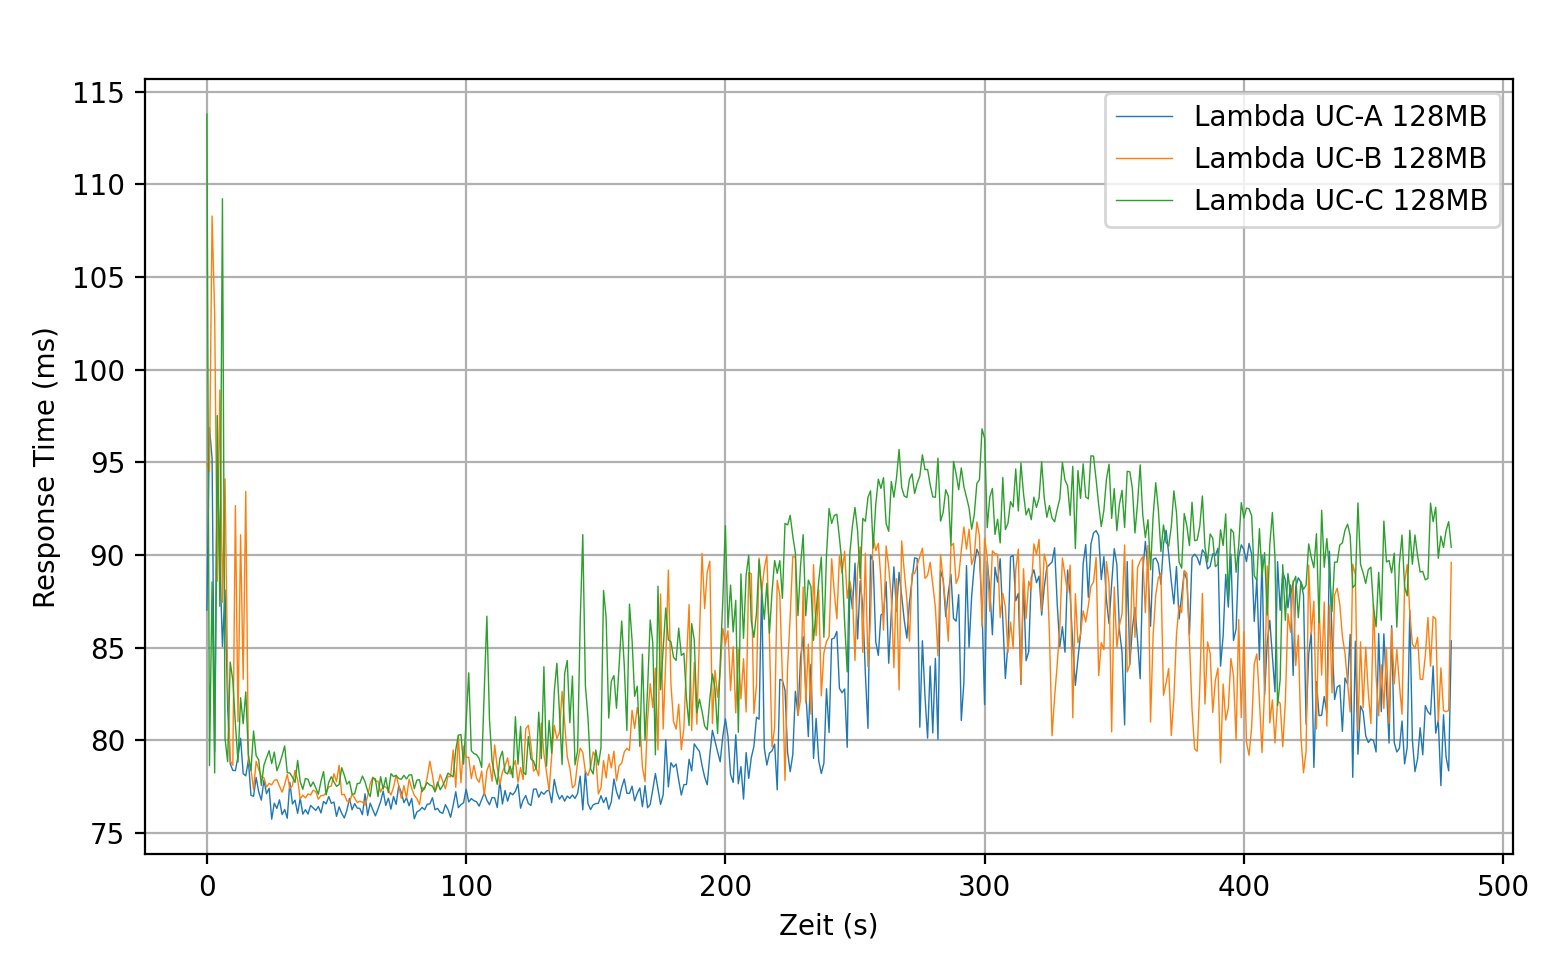
\includegraphics[width=\textwidth]{img/lambda128-load600-uc-comparison-new.png}
    \caption[Lambda Load-Test mit 600 VUs Verlauf Vergleich]{Lambda Load-Test mit 600 VUs Verlauf Vergleich}
    \label{fig:lambda128-load600-uc-comparison}
\end{figure}

Es ist zu erkennen, dass alle Use-Cases einen generell ähnlichen Verlauf haben. Use-Case A mit nur einem Endpunkt weist jedoch überwiegend die geringste Antwortzeit auf. Die Linie von Use-Case B liegt nur leicht über der des ersten Use-Case und übertrifft diesen sogar teilweise gegen Ende des Vergleichs. Use-Case C mit den meisten Endpunkten weist auch die höchsten Antwortzeiten auf und erreicht mit über 95ms ein in etwa 5ms höheres Maximum als die anderen beiden Use-Cases.  


\section{Andere Konfigurationen (\hyperref[tab:research-questions]{RQ3})}
Als nächstes sollen Container und Lambda-Funktionen mit einer CPU- und Speicher-Größe von 256 und 512 Megabyte untersucht werden. Ziel dessen ist es, Unterschiede zu den in der vorangegangenen Sektion getesteten Konfigurationen zu erkennen.

\subsection{Pipe-Clean Tests}
Für die Pipe-Clean Tests der Container konnte keine Veränderung zur 128MB Variante festgestellt werden. Die Antwortzeit bewegte sich im Median erneut um die 60ms und auch der Variationskoeffizient zeigte nur eine äußerst geringfügige Veränderung. Bei allen Konfigurationen und Use-Cases wurden 90 Prozent aller Anfragen innerhalb von 62ms beantwortet. Größere CPU- und Arbeitsspeicher-Werte hatten hier also keine Verbesserung der Performance zur Folge.
Abbildung \ref{fig:pipe-comparison} zeigt die aggregierten Metrik-Werte der Pipe-Clean Tests für die unterschiedlich großen Konfigurationen der Lambda-Funktionen.

\begin{figure}[H]
    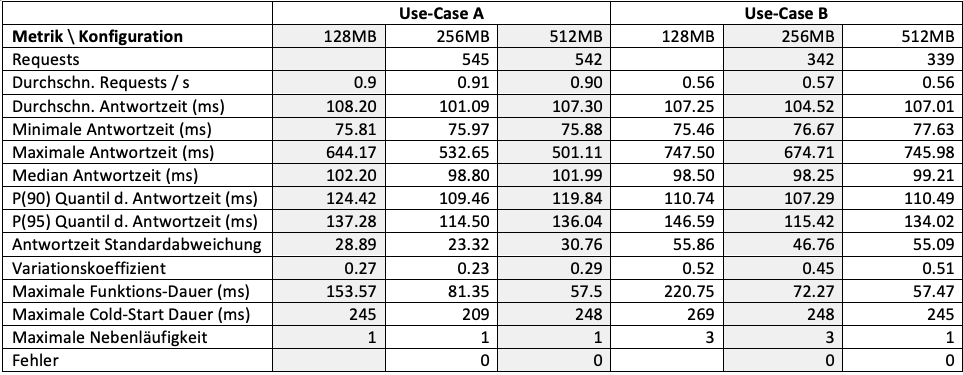
\includegraphics[width=\textwidth]{img/pipe-comparison.png}
    \caption[Vergleich der Pipe-Clean Tests für Lambda]{Vergleich der Pipe-Clean Tests für Lambda}
    \label{fig:pipe-comparison}
\end{figure}

Es wird deutlich, dass auch hier fast keine Unterschiede zwischen den drei Ausführungen bestehen. Die mediane Antwortzeit liegt für alle Use-Cases in etwa bei 100ms. Die P(90) und P(95) Quantile variieren leicht zwischen den Tests der verschiedenen Konfigurationen. Tendenziell sind sie bei den größeren Konfigurationen niedriger als bei den kleineren, es lässt sich jedoch kein eindeutiges Muster erkennen. Es können außerdem keine Unterschiede in der Coldstart-Dauer oder der Varianz festgestellt werden. 
Allerdings ist zu erkennen, dass die maximale Funktionsdauer bei den größeren Konfigurationen deutlich geringer wird und sich dem minimalen Wert von 50ms annähert. Während der Wert für Use-Case A und die 128MB Funktion noch bei 153,57ms liegt, sinkt er für die 256MB Funktion auf 81,35ms herab. Für die 512MB Variante liegt der Wert nur noch knapp über 60ms. Ähnliches ist für die anderen beiden Use-Cases festzustellen.

\subsection{Stress- und Load-Tests}
Zunächst soll der 256MB Container untersucht werden. Trotz der doppelt so großen Werte für Arbeitsspeicher und \ac{vCPU} konnte hier bei den Stress-Tests keine Verbesserung der maximalen Benutzer für die Container-Instanz erreicht werden. Genau wie der 128MB Container, begann die Antwortzeit des 256MB Containers für Use-Case A bei ca. 700 \acp{VU} stark anzusteigen. Für Use-Case B kam es ab ca. 900-1.100 \acp{VU} zum Anstieg der Antwortzeiten. Für Use-Case C wurde ein Limit von ca. 1.100-1.300 \acp{VU} erkannt. Damit ist kein großer Unterschied zu der 128MB Variante erkennbar.

Der Verlauf der Stress-Tests für der 128MB Serverless-Anwendung hatte gezeigt, dass eine größere Anzahl an Endpunkten zu höheren Antwortzeiten führen kann (vgl. Abbildung \ref{fig:lambda128-stress1000-comparison-graph}). Wie Abbildung \ref{fig:lambda256-stress1000-comparison-graph} für den Stress-Test mit bis zu 1.000 \acp{VU} zeigt, ist dies auch bei den 256MB Lambda-Funktionen der Fall. Allerdings scheint der Größenunterschied zwischen den Use-Cases im Vergleich zu der kleineren Konfiguration zurückgegangen zu sein. Auch bei dieser Abbildung werden die ersten 60 Sekunden nicht angezeigt, da die initial sehr hohen Antwortzeiten die Darstellung der Verläufe stark verzerren würde. 

\begin{figure}[H]
    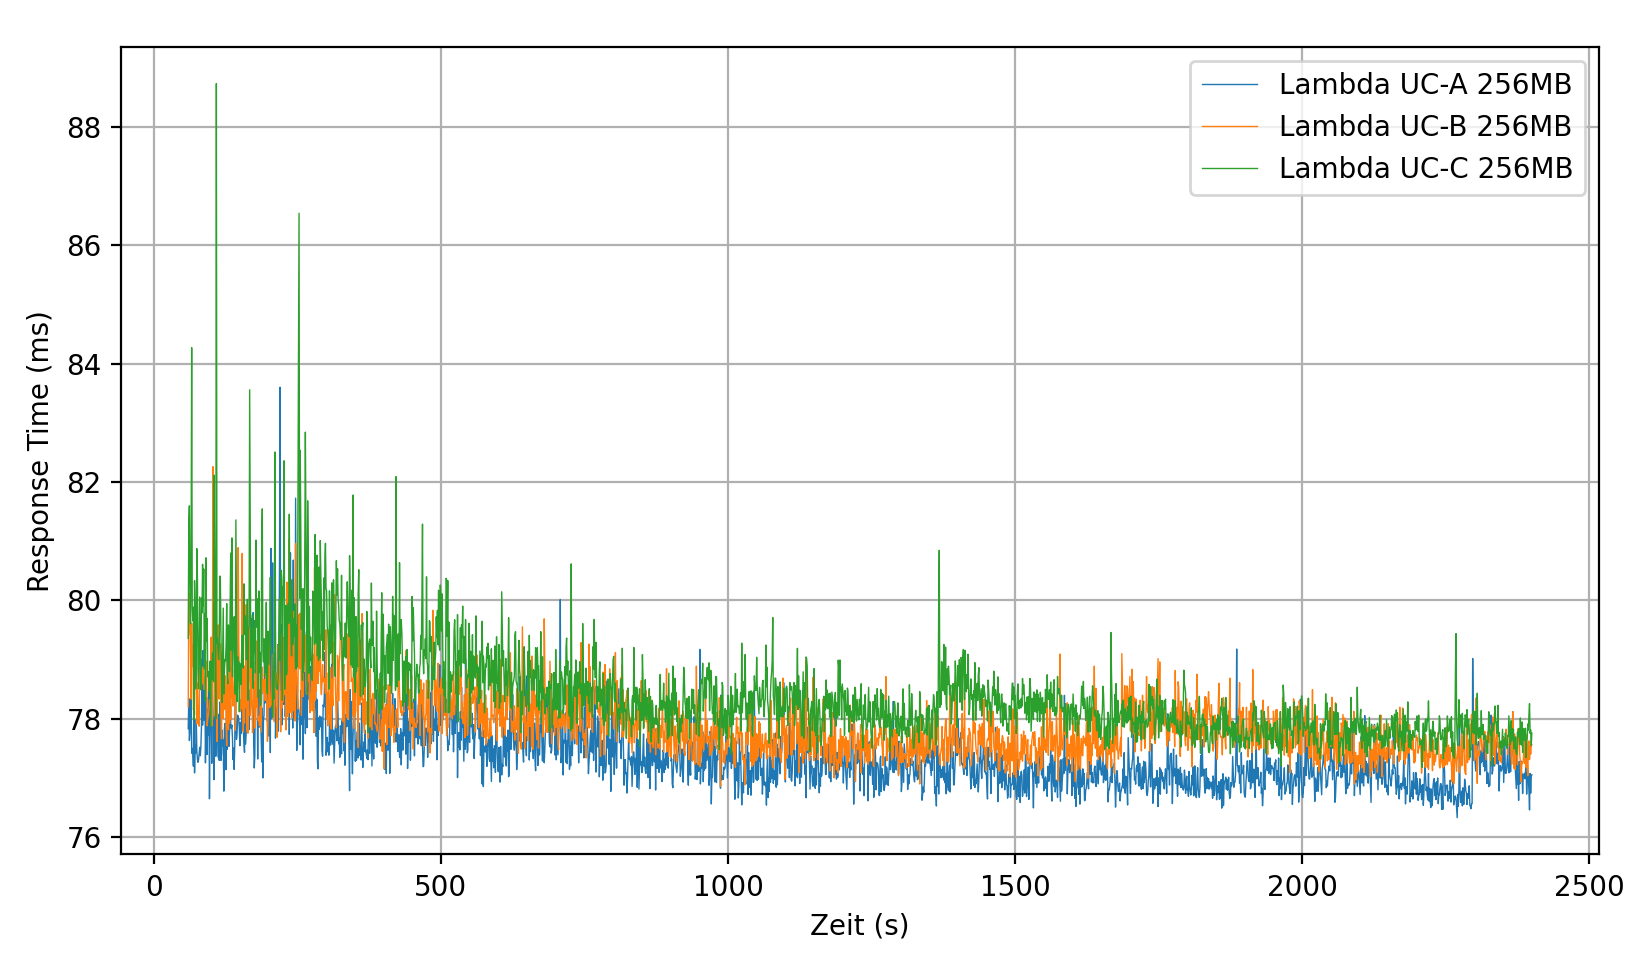
\includegraphics[width=\textwidth]{img/lambda256-stress1000-comparison-graph.png}
    \caption[Lambda 256MB Stress-Test mit 1.000 VUs Verlauf Vergleich]{Lambda 256MB Stress-Test mit 1.000 VUs Verlauf Vergleich}
    \label{fig:lambda256-stress1000-comparison-graph}
\end{figure}

Bei allen drei Use-Cases lagen die Antwortzeiten dennoch nahe um einen Median-Wert von ca. 78ms und es wurden 95 Prozent aller Anfragen in etwa 100ms verarbeitet. Bei der 128MB Variante reichte das P(95) Quantil noch von 114ms bis zu mehr als 122ms. Der Variationskoeffizient lag in allen Fällen bei 0,16 bis 0,18 und ist damit deutlich geringer als bei der kleineren Konfiguration, bei der er meistens 0,22 betrug, allerdings in einem Fall auch einen Wert von 0,64 erreichte. Damit ist eine deutliche Verbesserung der Performance und der Varianz in den Stress-Tests für die 256MB Variante festzustellen.

Im Anschluss wurden die Last- bzw. Spike Tests durchgeführt, um diese mit der 128MB Variante zu vergleichen. Als \ac{VU}-Limit wurde erneut 600 Benutzer festgelegt. Dies ermöglicht einen einfachen Vergleich der beiden Varianten.
Auch hier konnten für die Container-Anwendung keine Unterschiede zu der kleineren Konfiguration festgestellt werden. 

\begin{figure}[]
    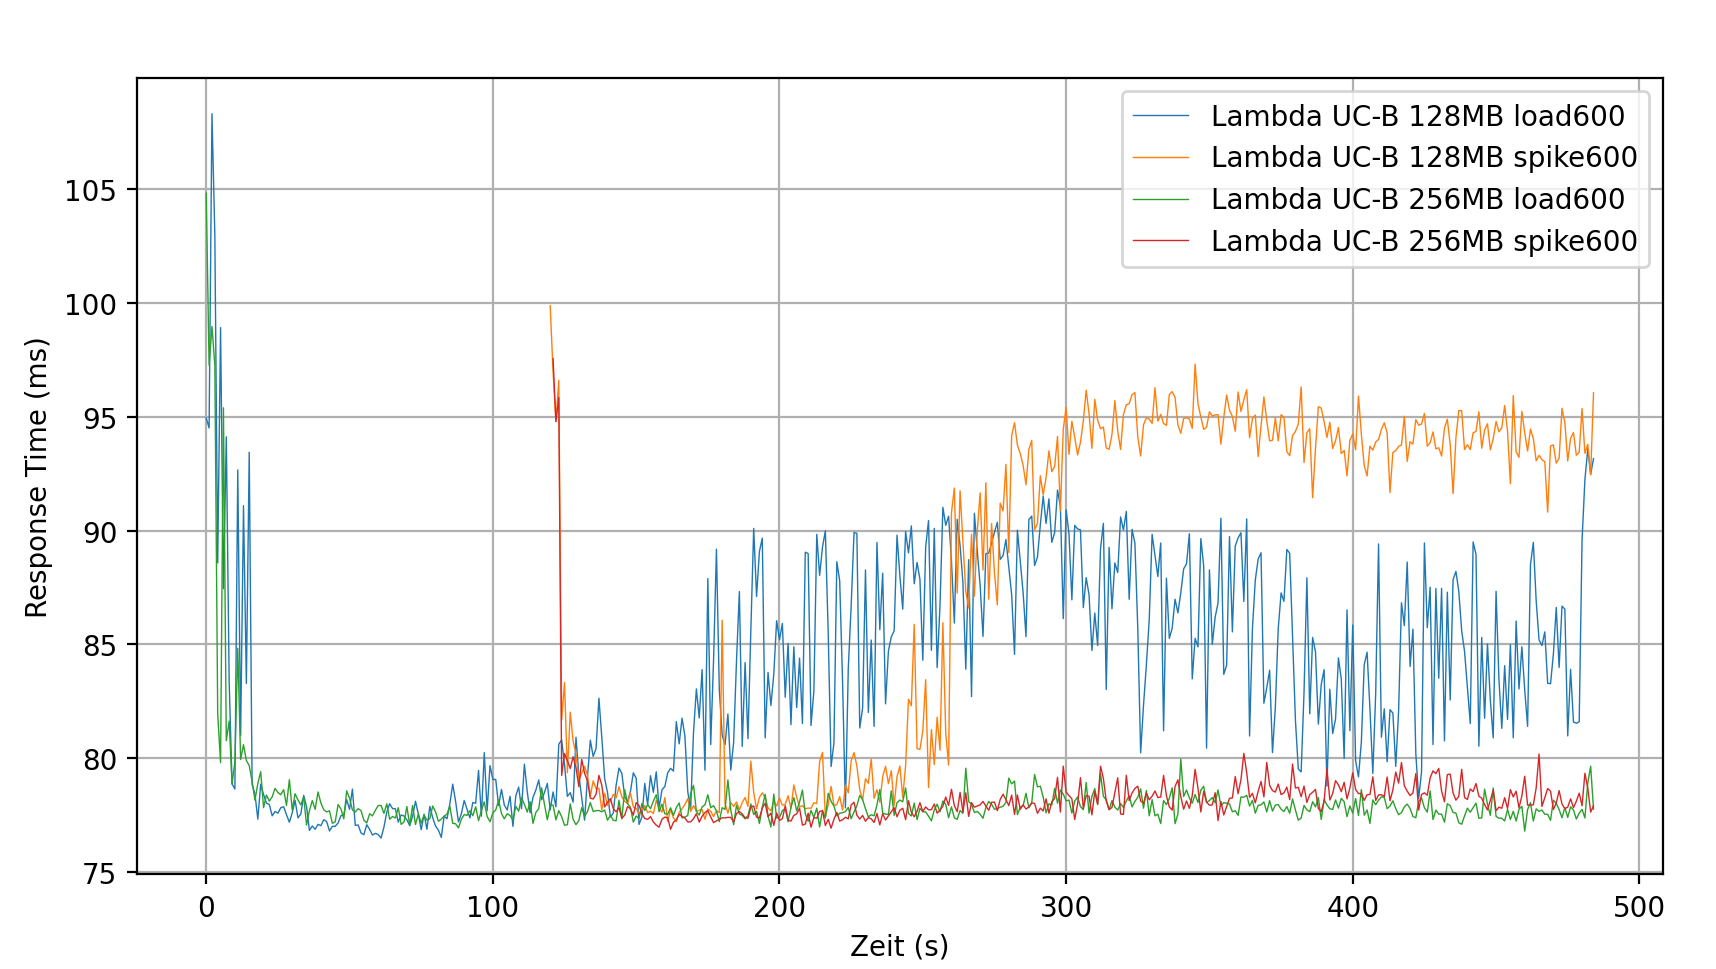
\includegraphics[width=\textwidth]{img/lambda128+256-ucb-load600-vs-spike600-graph.png}
    \caption[Lambda 128MB und 256MB Load- und Spike-Tests mit 600 VUs Verlauf Vergleich]{Lambda 128MB und 256MB Load- und Spike-Tests mit 600 VUs Verlauf Vergleich}
    \label{fig:lambda128+256-ucb-load600-vs-spike600-graph}
\end{figure}

Für die Lambda-Funktionen der Use-Cases A und B sind bei der 256MB Variante im Gegensatz zu der 128MB Konfiguration keine wesentliche Unterschiede zwischen den Load- und Spike Tests zu erkennen. Wie in Abbildung \ref{fig:lambda128+256-ucb-load600-vs-spike600-graph} für Use-Case B zu erkennen ist, sind die größeren Funktionen nahezu gar nicht von der Skalierung betroffen. Die Antwortzeit liegt, bis auf den anfänglichen Anstieg, beständig zwischen ca. 75 und 80ms. Im Vergleich zu der kleineren Variante, verkleinerte sich der Variationskoeffizient von 0,22 auf 0,17. Wie schon bei den Pipe-Clean Tests zu sehen war, sinkt auch hier die maximale Funktionsdauer von über 600ms bei 128MB auf unter 300ms ab. Bei den Antwortzeiten gab es ebenso eine geringfügige Verbesserung. Bei Coldstart-Dauer konnte dagegen keine Veränderung festgestellt werden.
Allein bei Use-Case C gibt es Unterschiede in den Antwortzeiten. Während der Wert des Medians sich bei den Load-Tests nur etwas über 78ms befindet, liegt er bei den beiden Durchläufen der Spike-Tests bei 88,46 und 84,26ms. Vermutlich ist dies auf vermehrte Coldstarts durch die größere Anzahl an Endpunkten zurückzuführen.
Bei den Load-Test-Durchläufen für Use-Case A wurden 69 bzw. 61 nebenläufige Funktionen registriert; bei den Spike-Tests waren es jeweils 62. Bei Use-Case B waren es 60 bzw. 58 und 57 bzw. 58. Die Tests für Use-Case C ergaben 53 bzw. 51 und 58 bzw. 55 parallele Funktionen. Damit liegt die Nebenläufigkeit für alle Use-Cases bei ähnlichen Werten im Vergleich zu den 128MB Funktionen.


Als nächstes sollen Container und Lambda-Funktionen mit einer CPU- und Speicher-Größe von 512 Megabyte untersucht werden. Ein Stress-Test des Containers mit bis zu 1.500 Benutzern ergab für Use-Case A, dass die Antwortzeit des Containers ab einer \ac{VU}-Anzahl von ca. 1.400 Benutzern deutlich zunimmt. Mit Eintreten der 1.400 Benutzer erreichte das Container-Cluster laut CloudWatch ebenso eine CPU-Auslastung von 100 Prozent. Dies bedeutet eine Verdoppelung des \ac{VU}-Limits zu den kleineren Varianten. Bei einem zweiten Test konnte für Use-Case A allerdings keine Veränderung der Antwortzeit festgestellt werden. Darum wurden weitere Stress-Tests mit bis zu 2.000 Benutzern getestet und ein \ac{VU}-Limit von ca. 1.600 identifiziert. Für Use-Case B musste ein weiterer Stress-Test ausgeführt werden, da bei 2.000 Benutzern nur eine CPU-Auslastung von 88\% erreicht werden konnte. Dieser wurde mit bis zu 2.500 Benutzern durchgeführt. Bei ca. 2.200-2.400 \acp{VU} wurde die maximale Auslastung des Containers erreicht. Ein weiterer Stress-Test mit bis zu 3.000 \acp{VU} ergab für Use-Case C ein Limit von ca. 2.800-3.000 Benutzern. Wie schon in früheren Tests konnte keine Veränderung der Container Antwortzeiten erkannt werden, bevor eine annähernde Vollauslastung des Prozessors erreicht wurde.

Im Anschluss an die Stress-Tests des Containers wurden diese mit den gleichen Konfigurationen gegen die Lambda-Anwendung durchgeführt. Dabei wurden einige Veränderungen zu den Stress-Tests der kleineren Varianten festgestellt. Beispielsweise schwankte die Median-Antwortzeit der Use-Cases B und C bei bis zu 2.000 Benutzern zwischen 81 und 88ms und fiel damit deutlich höher aus, als bei den Stress-Tests mit bis zu 1.000 Benutzern der 256MB Variante, bei der diese durchgehend zwischen 77 und 79ms gelegen hatte. Außerdem wurden bis zu 5ms Unterschiede in den Verläufen der gleichen Tests registriert. Der Abweichungskoeffizient erhöhte sich außerdem wieder auf Werte zwischen 0,19 und 0,28. Allein Use-Case A blieb sowohl bei der Median-Antwortzeit bei 77 bis 78ms und bei einem Variationskoeffizienten von 0,16 bzw. 0,17.

Die Load- und Spike-Tests wurden für die 512MB Konfiguration mit 1.200 \acp{VU} durchgeführt. Bei dem Fargate-Container konnte wie schon zuvor keine Unterschiede zwischen den beiden Tests festgestellt werden. Bis auf einige Ausreißer wurde wie schon bei den kleineren Konfigurationen für alle Use-Cases und für beide Anstiege eine Antwortzeit im Median von ca. 60ms festgestellt. Der Variationskoeffizient bewegt sich in den Testausführungen meist zwischen 0,03 und 0,05 und liegt damit nur geringfügig über den Werten der Pipe-Clean Tests. Bis auf eine höhere Anzahl der verarbeitbaren Anfragen konnten also keine Performance-Verbesserungen der 512MB Konfiguration festgestellt werden.

Die Load-Tests der 512MB Lambda-Funktionen bestätigten erneut, dass die Anzahl der Endpunkte einen Einfluss auf die Antwortzeiten hat. Es gab hier allerdings bei den Use-Cases A und B wie schon bei den Stress-Tests Unterschiede von einigen Millisekunden zwischen den Ausführungen des gleichen Anwendungsfalls. So war die beste Ausführung des Use-Case B besser als die schlechtere Ausführung des Use-Cases A. Die beste Variante des ersten Use-Cases war aber erneut besser als die performanteste Ausführung von Use-Case B. Der Use-Case mit den meisten Endpunkten schnitt wieder deutlich am unperformantesten ab.

Auch bei den Spike-Tests traten ähnliche Abweichungen wie bei den Load-Tests auf. Deshalb werden für die Analyse nur die jeweils besten Läufe betrachtet. Abbildung \ref{fig:lambda512-load1200-vs-spike1200-graph} zeigt den Verlauf der Load-Tests im Vergleich mit den Spike-Tests. 

Auch hier zeichnet sich der Einfluss der Anzahl der Endpunkte ab. Der Median von Use-Case B liegt mit 78ms zwar nur knapp über den 77,02ms von Use-Case A. Deutlicher ist aber der Abstand von Use-Case C, dessen Antwortzeiten sich fast durchgängig bei in etwa 85ms befinden. 
Wie schon bei der 256MB Konfiguration ist kein Unterschied zwischen den Load-Test Ausführungen der Use-Cases A und B und den korrespondierenden Spike-Tests erkennbar. Für Use-Case C kann in der 512MB Konfiguration das gleiche beobachtet werden. Es zeigt sich also trotz der doppelt so großen Benutzerzahl im Vergleich zu den kleineren Konfigurationen eine leichte Verbesserung des Skalierungsverhaltens.

\begin{figure}[H]
    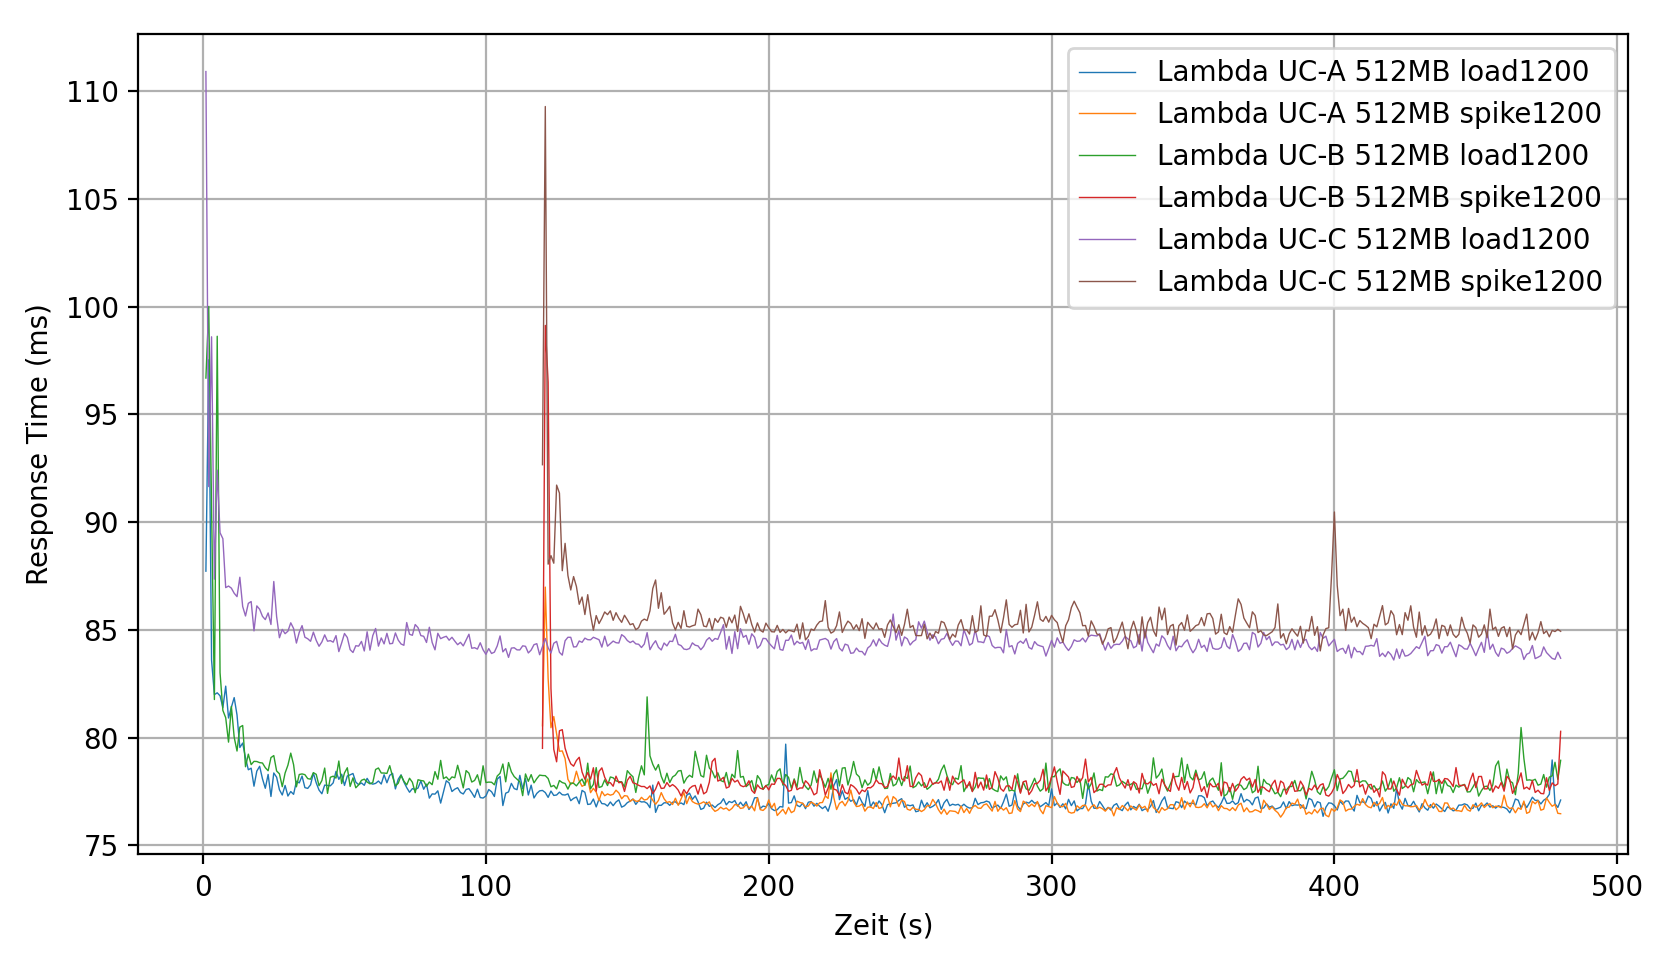
\includegraphics[width=\textwidth]{img/lambda512-load1200-vs-spike1200-graph.png}
    \caption[Lambda 512MB Load- und Spike-Tests mit 1.200 VUs Verlauf Vergleich]{Lambda 512MB Load- und Spike-Tests mit 1.200 VUs Verlauf Vergleich}
    \label{fig:lambda512-load1200-vs-spike1200-graph}
\end{figure}

\section{Mehrere Container (\hyperref[tab:research-questions]{RQ4})}
Für die Untersuchung inwiefern sich die Anzahl der aktiven Container auf die Performance auswirkt, wurde ein Test mit der Fargate 256MB Task-Definition durchgeführt. Dazu wurden zwei Container-Instanzen gestartet und erneut Stress-Tests unterzogen. Bei Use-Case A wurde das Limit der Virtuellen Benutzer bei ca. 1.500 erkannt. Use-Case B wies eine Belastungsgrenze zwischen 2.100 und 2.300 \acp{VU} auf. Beim dritten Anwendungsfall wurden in etwa. 2.800 bis 2.900 \acp{VU} registriert bevor die Performance degradierte. 
Damit liegen diese Werte sehr ähnlich an denen des 512MB Containers (siehe vorherige Sektion), bei dem Werte von 1.400, 2.200 bis 2.400 und 2.800 bis 3.000 \acp{VU} festgestellt wurden.

Im Anschluss wurden deshalb für die zwei 256MB Instanzen erneut Load-Tests mit bis zu 1.200 Benutzern durchgeführt, um eventuelle Performance Unterschiede zu der großen Konfiguration zu erkennen. Abbildung \ref{fig:fargate-2x256-vs-512-load1200-comparison} zeigt die Ergebnisse der Tests im Vergleich mit denen des 512MB Containers.

\begin{figure}[H]
    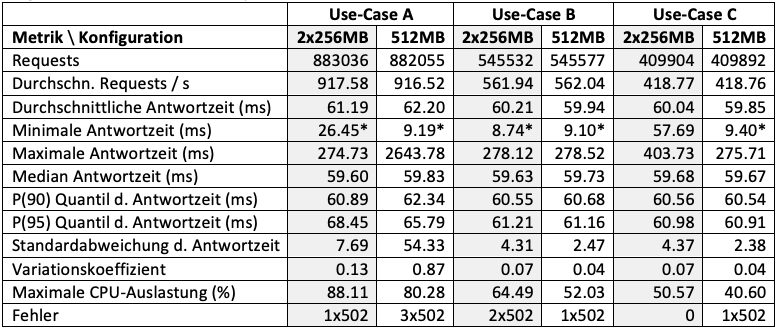
\includegraphics[width=\textwidth]{img/fargate-2x256-vs-512-load1200-comparison.png}
    \caption[Vergleich der Load-Tests für 2x256MB und 512MB mit 1.200 VUs]{Vergleich der Load-Tests für 2x256MB und 512MB mit 1.200 VUs}
    \label{fig:fargate-2x256-vs-512-load1200-comparison}
\end{figure}

Es wird deutlich, dass keine eindeutigen Unterschiede in der Performance zweier 256MB Instanzen zu einer einzelnen 512MB Instanz sichtbar werden. Beide Konfigurationen weisen sowohl ähnliche Requests pro Sekunde, als auch nahezu identische Antwortzeiten auf. Die Varianz ist bei allen Ausführungen äußerst niedrig und nur leicht über dem Niveau der Pipe-Clean Tests. Allein bei Use-Case A gab es größere Abweichungen vom Mittelwert, dieser wies aber auch in beiden Fällen die größte CPU-Auslastung auf. In der Auslastung des Clusters ist ebenfalls der größte Unterschied der beiden Konfigurationen zu erkennen. Bei allen Use-Cases lag diese bei den zwei Instanzen deutlich über der des einzelnen Containers. Bei Use-Case A waren es ca. acht Prozent, bei Use-Case B mehr als zwölf und bei Use-Case C ca. zehn Prozent mehr. 


\section{Kosten}
\label{sec:kosten}
In dieser Sektion sollen die Kostenmodelle der in dieser Arbeit getesteten Technologien untersucht und verglichen werden. Dabei wird sich erneut auf \ac{AWS} beschränkt. Es kann daher bei anderen Public-Cloud Anbietern deutliche Unterschiede geben. Da es zwischen den einzelnen \ac{AWS} Regionen ebenso Preisunterschiede bei der Nutzung des gleichen Services gibt, beziehen sich die folgenden Ausführungen ausschließlich auf die Region Frankfurt (eu-central-1).

\subsection{Container}
Da viele verschiedene Wege existieren Container-Anwendungen in der Public-Cloud zu betreiben, wird für die Kosten-Schätzung nur der Betrieb der Anwendung mit \ac{ECS} und dem Starttyp Fargate betrachtet, wie er in dieser Arbeit verwendet wurde.

Bei Fargate wird die Abrechnung in die gewählte Arbeitsspeicher und \ac{vCPU}-Größe unterteilt. Der Preis für ein Arbeitsspeicher Gigabyte pro Stunde beträgt aktuell 0,00511\$ und der für ein \ac{vCPU} pro Stunde 0,04656\$\cite{noauthor_aws_nodate-2}. Die Formel \ref{fargate-kosten-formel} zeigt die Berechnung der Kosten für ein Fargate-Cluster.


\begin{equation}
Kosten = Tasks * Stunden * Tage * (SpeicherGB * 0,00511\$ + AnzahlvCPUs * 0,04656\$)
\label{fargate-kosten-formel}
\end{equation}

Es wird davon ausgegangen, dass mindestens ein Task dauerhaft laufen muss, damit der Service erreichbar bleibt. Für die in dieser Arbeit verwendete 128MB und 256MB Konfigurationen (mit 0.25 \ac{vCPU}) ergäben sich für einen laufenden Task pro Monat (30 Tage) und Dauerbetrieb (24 Stunden pro Tag) Kosten von: \\

$Kosten = 1 * 24 * 30 * (0,5 * 0,00511\$ + 0,25 * 0,04656\$) = 10,22\$$ \\

Dieser Wert konnte mit den in dieser Arbeit durchgeführten Tests bestätigt werden, da für jeden Tag Kosten von 0,34\$ für die Nutzung des Clusters von \ac{AWS} abgeführt wurden. Bei 30 Tagen Laufzeit ergeben sich damit tatsächlich Gesamtkosten von 10,2\$.

Aus der Formel lässt sich ableiten, dass sich für eine n-fache Anzahl an Tasks auch die n-fachen Kosten pro Monat ergeben. Variationen in der Anzahl der Tasks aufgrund von (Auto-) Skalierung sind unmöglich vorauszusagen und werden daher nicht betrachtet.

Zusätzlich zu den Fargate Kosten sind noch Gebühren für die Nutzung des \acp{ELB} fällig, dessen Nutzung bei der Verwendung mehrerer Instanzen unabdingbar ist. Für einen Application Load Balancer fallen pro angefangener Stunde Kosten von 0,027\$ an. Das ergibt für 30 Tage Kosten von 19,44\$. Zusätzlich fallen noch Gebühren für die Auslastung des Load-Balancers an; bspw. für die aktiven Verbindungen pro Minute\cite{noauthor_preise_nodate}. Auch diese können nicht vorausgesagt werden und werden daher bei der Berechnung vernachlässigt.

Die folgende Übersicht zeigt die monatlichen Fixkosten einer Instanz für die unterschiedlichen in dieser Arbeit verwendeten Konfigurations-Größen inklusive Nutzung eines Application Load Balancers:

\begin{itemize}
    \item 128MB = 0,5GB und 0,25 vCPU $\Rightarrow$ 10,22\$ + 19,44\$ (\ac{ELB}) = 29,66\$
    \item 256MB = 0,5GB und 0,25 vCPU $\Rightarrow$ 10,22\$ + 19,44\$ (\ac{ELB}) = 29,66\$
    \item 512MB = 1  GB und 0,5  vCPU $\Rightarrow$ 20,44\$ + 19,44\$ (\ac{ELB}) = 39,88\$
    \item 1024MB = 2 GB und 1    vCPU $\Rightarrow$ 40,88\$ + 19,44\$ (\ac{ELB}) = 60,32\$
\end{itemize}

\noindent
Kosten für Skalierung und die Nutzung des Load-Balancers müssen, wie bereits beschrieben, noch separat hinzugerechnet werden. Es wird deutlich, dass die Kosten für zwei 256MB Container der eines 512MB Containers entsprechen. Genau so ergeben zwei 512MB Container die gleichen Kosten eines einzelnen 1024MB Containers. 

\subsection{Lambda}
\label{subsec:kosten-lambda}
Die Ausführung von Lambda-Funktionen wird nach der Ausführungszeit in Millisekunden abgerechnet. Dabei wird die Zeit für einen Cold-Start mit einberechnet. Auch die konfigurierte Arbeitsspeichergröße fließt mit in das Ergebnis ein. Derzeit berechnet \ac{AWS} in der Region Frankfurt Kosten von 0,0000166667 US-Dollar pro Gigabyte-Sekunde (GB-Sekunde). Zusätzlich \linebreak müssen pro einer Millionen Ausführungen einer Funktion im Monat noch einmal 0,20 US-Dollar Anforderungsgebühren gezahlt werden. \ac{AWS} bietet ein kostenloses Nutzenkontingent von 400.000 Aufrufen pro Funktion im Monat an\cite{noauthor_lambda_nodate-2}.

Für die Ausführung der Lambda-Funktionen wird ein Event-Auslöser für REST-Anfragen benötigt. Dazu wurde in dieser Arbeit der Amazon API-Gateway Service verwendet, welches eingehende Requests auf die vorgesehene Lambda-Funktion weiterleitet. Für die Verwendung des API-Gateways fallen zusätzliche Kosten an. Bei Nutzung des Serverless-Frameworks wird automatisch eine API des Typs REST erstellt. Es fallen für diesen API-Typ Kosten von 3,70 Euro pro einer Millionen Aufrufe an. Diese werden für jede API insgesamt berechnet und gelten damit nicht für jede einzelne aufgerufene Lambda-Funktion. Es gibt Vergünstigungen ab 333 Millionen Aufrufen im Monat. In dieser Arbeit werden keine Caching Mechanismen des API-Gateways verwendet. Werden diese in den Einstellungen der API aktiviert, fallen zusätzliche Kosten an. \ac{AWS} bietet für das API-Gateway ein kostenloses Nutzenkontingent von einer Millionen Aufrufen im Monat\cite{noauthor_amazon_nodate-2}. Formel \ref{lambda-kosten-formel} zeigt die zusammengesetzte Berechnung der Gesamtkosten für eine Lambda-Funktion.

\begin{equation}
\begin{split}
Kosten = Aufrufe * \left(\frac{LaufzeitMs}{1000ms} * \frac{FunktionsMb}{1024Mb} * 0,0000166667\$ + \frac{0,20\$ + 3,70\$}{1.000.000}\right)
\end{split}
\label{lambda-kosten-formel}
\end{equation}

In den Tests der vorherigen Kapitel lag die Antwortzeit der Lambda-\linebreak Funktionen im Median oft um einen Wert von ca. 80ms. Unter Nutzung der Kostenformel \ref{lambda-kosten-formel} ergibt sich für eine Millionen Aufrufe einer einzigen Lambda-Funktion mit einer Größe von 128MB und dieser Laufzeit, ohne Einberechnung der kostenlosen Nutzenkontingente, ein Preis von: \\

\noindent
$Kosten = 1.000.000 * \left(\frac{80}{1000}*\frac{128}{1024} * 0,0000166667\$ + \frac{0,20\$ + 3,70\$}{1.000.000}\right) = 4,07\$$ \\

Die nachfolgende Tabelle zeigt die Kosten von unterschiedlichen Funktionsgrößen pro einer Millionen Aufrufe und für eine Laufzeit von 80ms.

\begin{table}[H]
\label{lambda-kosten-70ms-1000000aufrufe}
\begin{tabular}{lllll}
\hline
Funktionsgröße & 128MB   & 256MB   & 512MB   & 1024MB  \\ \hline
Kosten         & 4,07 \$ & 4,23 \$ & 4,57 \$ & 5,23 \$ \\ \hline
\end{tabular}
\end{table}

Da bei Lambda im  Gegensatz zu \ac{ECS} mit Fargate nur die tatsächlich aktive Zeit der Funktion berechnet wird, lässt sich grob abschätzen, wie viele Funktionsaufrufe zu dem gleichen Preis der Nutzung eines Fargate-Containers möglich sind (siehe vorherige Sektion). Es wird im folgenden davon ausgegangen, dass eine Funktion eine Laufzeit von 1ms bis zu 100ms hat. Die Umstellung der Kostenformel \ref{lambda-kosten-formel} ergibt Formel \ref{lambda-aufrufe-formel} zur Berechnung der Aufrufe bei Angabe der Kosten.

\begin{equation}
\label{lambda-aufrufe-formel}
Aufrufe = \frac{Kosten}{\frac{LaufzeitMs}{1000ms} * \frac{FunktionsMb}{1024Mb} * 0,0000166667\$ + \frac{0,20\$ + 3,70\$}{1.000.000}}
\end{equation}

Abbildung \ref{fig:lambda-max-invocations} zeigt das Ergebnis der Berechnungen. Die Werte der 128MB und 256MB Funktionen stimmen überein, da der Preis für die Fargate Konfiguration identisch ist.

\begin{figure}[H]
    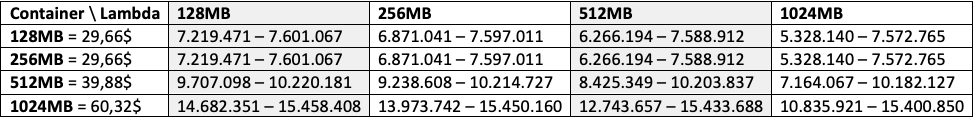
\includegraphics[width=\textwidth]{img/lambda-max-invocations.png}
    \caption[Anzahl der Aufrufe von Lambda-Funktionen dem Monatspreis von Fargate entsprechend]{Anzahl der Aufrufe von Lambda-Funktionen dem Monatspreis von Fargate entsprechend}
    \label{fig:lambda-max-invocations}
\end{figure}

Der jeweils linke Wert in den Tabellenzellen gibt dabei die minimale Anzahl der Aufrufe an, wenn jeder Funktionsaufruf bei 100ms liegt. Der rechte Wert ist der für eine Funktions-Dauer von 1ms und beschreibt damit den maximal möglichen Wert, da Lambda immer mindestens eine Millisekunde abrechnet\cite{noauthor_lambda_nodate}. Es wird deutlich, dass schon für die Nutzung eines 128MB Containers im Monat zwischen sieben und fast acht Millionen Aufrufe einer Lambda-Funktion möglich sind. Das entspricht mehr als 240.000 Aufrufen täglich. Je größer der genutzte Container wird, desto größer wird auch die Anzahl der mit einer gleichwertigen Lambda-Funktion möglichen Aufrufe. Bei einem 512MB Container sind so schon zwischen acht und zehn Millionen Aufrufe einer 512MB Lambda-Funktion monatlich möglich. Bei einem 1024MB Container sind es sogar zwischen 10,8 und fünfzehn Millionen, was zwischen 360.000 und 500.000 Aufrufen täglich entspricht.
Es muss darauf hingewiesen werden, dass die Kosten deutlich abhängig sind von der tatsächlichen Nutzung der Anwendung, da dadurch viele oder wenige Coldstarts ausgelöst werden können, die unter Umständen einige hundert Millisekunden dauern können.